\documentclass[pdf]{prosper}
\usepackage{amsmath}
\DeclareSymbolFont{AMSb}{U}{msb}{m}{n}
\DeclareMathSymbol{\natural}{\mathbin}{AMSb}{"4E}
\DeclareMathSymbol{\integer}{\mathbin}{AMSb}{"5A}
\DeclareMathSymbol{\real}{\mathbin}{AMSb}{"52}
\DeclareMathSymbol{\rational}{\mathbin}{AMSb}{"51}
\DeclareMathSymbol{\I}{\mathbin}{AMSb}{"49}
\DeclareMathSymbol{\complex}{\mathbin}{AMSb}{"43}


\usepackage[all]{xy}
\usepackage{graphicx}
\title{A tale of two DVCSes}
\subtitle{darcs versus git}
\author{Miles Gould}
\institution{University of Edinburgh \\
miles@assyrian.org.uk \\
@pozorvlak \\
pozorvlak.livejournal.com \\
github.com/pozorvlak}
\begin{document}
\maketitle

% Overview

\begin{slide}{Overview}
\begin{itemize}
\item Both highly distributed
\item Both allow rewriting of unpublished history
\item Many features borrowed from each other
\item But under the hood, almost totally different
\item Similar terminology hides differences
\item Different terminology hides similarities
\end{itemize}
\end{slide}

\begin{slide}{Git}
\begin{itemize}
\item Written by some Finnish dude in 2005 as a side-project
\item C/shell/Perl/Python/...
\item content-addressable filesystem
\begin{itemize}
	\item everything indexed by hash of contents
	\item a version is a tree of blobs
	\item a commit is a tree, pointers to parents, metadata
	\item diffs calculated as needed
\end{itemize}
\item Inspired by Monotone (but faster)
\item History is a DAG of commits (snapshots).
\end{itemize}
\end{slide}

\begin{slide}{Darcs}
\begin{itemize}
\item Written by physicist David Roundy in 2003
\item Initially C++, rewritten in Haskell
\item A repository is an \emph{unordered collection of patches}
\item A patch is an \emph{abstract atomic change}
\item To apply a patch to a repo, must calculate a concrete \emph{effect}
\item Potential for high-level patch types
\item Patches may \emph{depend} on other patches
\end{itemize}
\end{slide}

% Merging

\begin{slide}{Merging in git}
\[
\xymatrix{
& \bullet \\
A \ar@{-->}[ur] & & B \ar@{-->}[ul] \\
& M \ar[ul] \ar[ur]
}
\]
\end{slide}

\begin{slide}{A more complex merge in git}
\[
\xymatrix{
& \bullet \\
A \ar@{-->}[ur] & & B \ar@{-->}[ul] \\
\\
M1 \ar[uu] \ar[uurr]
&& M2 \ar[uull] \ar[uu] \\
& \bullet \ar[ul] \ar[ur]
}
\]
\end{slide}

\begin{slide}{Rebasing in git}
\[
\xymatrix{
& \bullet \\
A & & B \ar@{-->}_{a'}[ul] \\
& M \ar[ul]^a \ar[ur]
}
\]
\end{slide}

\begin{slide}{Merging in darcs}
\[
\xymatrix{
& \bullet \ar@{-->}[dl]^*{\object{\scriptstyle{B^{-1\prime}}}} \\
\bullet \ar@/^1pc/[ur]^{B'}
& & \bullet \ar@/^1pc/[dl]^*{\object{\scriptstyle{B^{-1}}}} \ar[ul]_{A'} \\
& \bullet \ar[ul]^A \ar[ur]^B
}
\]
\begin{itemize}
\item Looks a lot like a rebase
\item But no false positives - if it succeeds, it's correct
\item Magic hidden in commutators - need one for each pair of patch types
\item Can take exponential time in case of conflicts
\end{itemize}
\end{slide}

% Cherry-picking

\begin{slide}{Cherry-picking in git}
\[
\xymatrix{
	\bullet \\
	\bullet \ar@{--}[u]^{a'} && \bullet \\
	\bullet \ar[u] && \bullet \ar[u] \\
	\bullet \ar[u] && \bullet \ar[u]_a \\
	& \bullet \ar[ul] \ar[ur]
}
\]
\end{slide}

\begin{slide}{Cherry-picking in darcs}
\[
\xymatrix{
	&& \bullet \\
	\bullet && \bullet \ar[u]_a \\
	\bullet \ar[u] && \bullet \ar[u] \\
	\bullet \ar[u] && \bullet \ar[u]_b \\
	& \bullet \ar[ul] \ar[ur]
}
\]
\end{slide}

\begin{slide}{Cherry-picking in darcs}
\[
\xymatrix{
	&& \bullet \\
	\bullet && \bullet \ar[u] \\
	\bullet \ar[u] && \bullet \ar[u]_{} \\
	\bullet \ar[u] && \bullet \ar[u]_{a'} \\
	& \bullet \ar[ul] \ar[ur]_{b'}
}
\]
\end{slide}

\begin{slide}{Cherry-picking in darcs}
\[
\xymatrix{
	\bullet \\
	\bullet \ar@{-->}[u]^{a''} && \bullet \\
	\bullet \ar@{-->}[u]^{b''} && \bullet \ar[u] \\
	\bullet \ar[u] && \bullet \ar[u] \ar@{-->}[uuull] \\
	\bullet \ar[u] && \bullet \ar[u]_{a'} \\
	& \bullet \ar[ul] \ar[ur]_{b'}
}
\]
\end{slide}

% Branching

\begin{slide}{Branching in git}
\begin{itemize}
\item Autoincrementing named pointer to a commit
\item Many branches in one repo
\item Cheap to make
\item Workflow encourages ``topic branches''
\end{itemize}
\end{slide}

\begin{slide}{Branching in darcs}
\begin{itemize}
\item No good story for branching
\item Must create a whole new repo
\item Or use ``spontaneous branches''
\begin{itemize}
\item Not spontaneous
\item Not branches
\item Ugh!
\end{itemize}
\item But less need for topic branches
\end{itemize}
\end{slide}

% Rosetta Stone

\overlays{2}{
\begin{slide}{A git/darcs Rosetta Stone}
	\begin{center}
\onlySlide*{1}{
	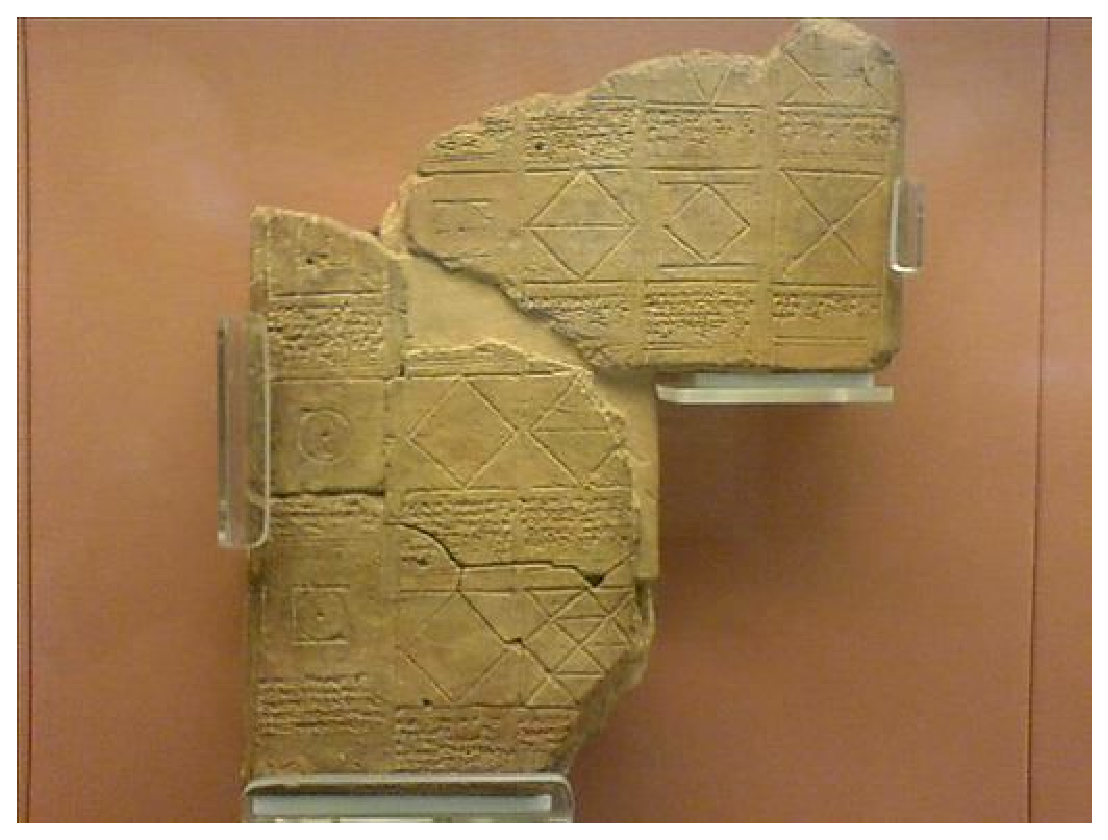
\includegraphics[width=8cm]{babylon.eps}
}
\fromSlide{2}{
	\begin{tabular}{ | p{5cm} | p{5cm} | }
	\hline
	\textbf{git} & \textbf{darcs} \\
	\hline
	long-lived branch & repository \\
	\hline
	commit	& collection of patches \\
	\hline
	rebase --interactive & ``preparation branch'' \\
	\hline
	topic branch	& patch \\
	\hline
	user specifies patch dependencies by branching
	& patch dependencies calculated optimistically by system \\
	\hline
	\end{tabular}
}
\end{center}
\end{slide}
}

% So why did git win?

\begin{slide}{So why has git (largely) won?}
Darcs is two years older, but has much less penetration.

In the early days, darcs suffered from
\begin{itemize}
\item poor performance
\item overly-high concept
\item poor documentation
\item "It's written in Haskell and works just like quantum mechanics! Here,
read this academic paper with equations in six colours!"
\end{itemize}
These screwed it before it could gain critical mass.
\end{slide}

\end{document}
